\chapter{多模态：理解与生成}
\label{chap:multimodal}

\begin{keybox}[两个方向，三个问题]
多模态模型有两个方向。理解方向把图像、视频或音频编码成表示，交给语言模型生成文字；生成方向以文字为条件，输出图像、视频或音频。两个方向都要回答三个问题：模态用什么 token 表示，条件从网络的哪个位置进入，用什么损失训练两者的对应关系。理解需要语义表示，生成需要能还原像素的表示，这一差别贯穿全章。
\end{keybox}

本章按信息流的顺序展开。第 \ref{sec:visual-tokens} 节把图像和视频变成 token 序列；第 \ref{sec:clip} 节用对比学习把图像与文本放进同一个表示空间，并从能量和互信息两个角度说明它优化的量；第 \ref{sec:vlm} 节把视觉 token 接进语言模型；第 \ref{sec:conditional-generation} 节反过来，以文本为条件生成图像和视频；第 \ref{sec:unified-multimodal} 节讨论把理解与生成放进同一个网络时遇到的矛盾。

\section{视觉 token 化：图像和视频怎样变成序列}
\label{sec:visual-tokens}

前面处理的是文字序列。要复用 Transformer 处理图像，需要先把二维像素变成一组向量，同时保留空间位置。视觉 Transformer（Vision Transformer，ViT）把图像切成固定大小的 patch，再把这些 patch 当作序列的 token。对大小为 \(H\times W\times 3\) 的图像，patch 边长为 \(P\) 时，patch 数为 \(N=(H/P)(W/P)\)；每个 \(P\times P\times3\) patch 展平成向量后，经线性投影变成 \(d_v\) 维 visual token~\cite{dosovitskiy2021vit}。另加入一个 CLS token，用于收集整幅图像的信息：
\begin{equation}
 u_i=W_{\mathrm{patch}}\operatorname{vec}(\operatorname{patch}_i)+b_{\mathrm{patch}},
 \qquad U_0=[u_{\mathrm{CLS}},u_1,\ldots,u_N]+P_{\mathrm{pos}}.
\end{equation}
其中 \(P_{\mathrm{pos}}\) 为位置向量。然后 \(U_0\) 进入普通 Transformer encoder。与语言 decoder 不同，ViT 使用双向自注意力：每个 patch 可以读取所有其他 patch；CLS token 的输出或所有 patch 的池化结果作为整幅图像的表示。训练目标可以是图像分类交叉熵，也可以是下一节的图文对比损失。

\textbf{分辨率与 token 数。}patch 数 \(N=HW/P^2\) 随分辨率平方增长，自注意力的计算和激活显存又随 \(N^2\) 增长。例如 \(P=14\) 时，\(336\times336\) 的图像给出 \(24\times24=576\) 个 patch，\(672\times672\) 的图像给出 2304 个。实际系统用两类办法控制 token 数。一是按图像的实际分辨率和长宽比决定 patch 网格，或把大图切成若干块分别编码，再附一张缩小的全图提供整体布局，避免统一缩放丢掉细节。二是在编码之后合并相邻 patch：把 \(2\times2\) 个相邻 patch 的特征拼成一个 \(4d_v\) 维向量，再用 MLP 投影回所需维度，token 数降为四分之一。合并保留了局部内容，只是每个 token 覆盖的面积变大；空间分辨率与 token 预算之间的取舍并没有消失。

\textbf{二维与时空位置。}语言序列只有一个位置下标，图像 patch 有行、列两个下标，视频 patch 还有帧号。第 \ref{sec:rope} 节的 RoPE 可以推广到多个下标。先把它的旋转矩阵写成分块形式：把每个 head 的 \(d\) 维 query 和 key 按相邻两维分成 \(d/2\) 个维度对，第 \(j\) 对记为 \(q^{(j)}=(q_{2j+1},q_{2j+2})\in\R^2\)（\(k^{(j)}\) 同理），配一个固定频率 \(\theta_j=b^{-2j/d}\)，常取 \(b=10^4\)。位置 \(m\) 处的旋转是块对角矩阵
\begin{equation}
 R_m=\diag\bigl(\rho(m\theta_0),\ldots,\rho(m\theta_{d/2-1})\bigr),
 \qquad
 \rho(\varphi)=\begin{pmatrix}\cos\varphi&-\sin\varphi\\ \sin\varphi&\cos\varphi\end{pmatrix}.
\end{equation}
二维旋转满足 \(\rho(\alpha)^\mathsf T\rho(\beta)=\rho(\beta-\alpha)\)，所以注意力 logit 按维度对拆成 \(d/2\) 项之和：
\begin{equation}
 (R_mq)^\mathsf T(R_nk)=\sum_{j=0}^{d/2-1}\bigl(q^{(j)}\bigr)^\mathsf T\rho\bigl((n-m)\theta_j\bigr)k^{(j)}.
 \label{eq:rope-pairs}
\end{equation}
每个维度对只感受到一个角度，即本对频率乘以位置差。

多模态旋转位置编码（Multimodal RoPE，M-RoPE）不改变维度对的划分，也不改变每一对的频率 \(\theta_j\)，只改变每一对旋转时乘的是哪个位置下标。位置换成三元组 \(p=(t,h,w)\)，分别是帧号、行号和列号；\(d/2\) 个维度对按编号分成连续的三组，第一组乘帧号 \(t\)，第二组乘行号 \(h\)，第三组乘列号 \(w\)。以 \(d=12\) 为例，6 个维度对的旋转角如下：
\begin{center}\small
\begin{tabular}{lcccccc}
\toprule
维度对 \(j\) & 0 & 1 & 2 & 3 & 4 & 5\\
对应的 query 分量 & \(q_1,q_2\) & \(q_3,q_4\) & \(q_5,q_6\) & \(q_7,q_8\) & \(q_9,q_{10}\) & \(q_{11},q_{12}\)\\
\midrule
一维 RoPE，位置 \(m\) & \(m\theta_0\) & \(m\theta_1\) & \(m\theta_2\) & \(m\theta_3\) & \(m\theta_4\) & \(m\theta_5\)\\
M-RoPE，图像 patch \((t,h,w)\) & \(t\theta_0\) & \(t\theta_1\) & \(h\theta_2\) & \(h\theta_3\) & \(w\theta_4\) & \(w\theta_5\)\\
M-RoPE，文本 token \((m,m,m)\) & \(m\theta_0\) & \(m\theta_1\) & \(m\theta_2\) & \(m\theta_3\) & \(m\theta_4\) & \(m\theta_5\)\\
\bottomrule
\end{tabular}
\end{center}
图像 patch 的前两对只随帧号转动，中间两对只随行号转动，最后两对只随列号转动。一般地，记三组的编号集合为 \(J_t,J_h,J_w\)，第 \(j\) 对的旋转角和整体旋转矩阵为
\begin{equation}
 \varphi_j(p)=
 \begin{cases}
 t\,\theta_j, & j\in J_t,\\
 h\,\theta_j, & j\in J_h,\\
 w\,\theta_j, & j\in J_w,
 \end{cases}
 \qquad
 R_p=\diag\bigl(\rho(\varphi_0(p)),\ldots,\rho(\varphi_{d/2-1}(p))\bigr).
 \label{eq:mrope}
\end{equation}
Qwen2-VL 中 \(d=128\)，64 个维度对按 16、24、24 分给 \(t,h,w\)~\cite{wang2024qwen2vl}。

logit 的“三段”来自式 \eqref{eq:rope-pairs} 的求和。那里的 \(d/2\) 项各对应一个维度对；把同一组的项归在一起，位置 \(p\) 的 query 与位置 \(p'\) 的 key 之间的 logit 就是
\begin{equation}
 (R_pq)^\mathsf T(R_{p'}k)
 =\sum_{j\in J_t}\bigl(q^{(j)}\bigr)^\mathsf T\rho(\Delta t\,\theta_j)k^{(j)}
 +\sum_{j\in J_h}\bigl(q^{(j)}\bigr)^\mathsf T\rho(\Delta h\,\theta_j)k^{(j)}
 +\sum_{j\in J_w}\bigl(q^{(j)}\bigr)^\mathsf T\rho(\Delta w\,\theta_j)k^{(j)},
\end{equation}
其中 \((\Delta t,\Delta h,\Delta w)=p'-p\)。在 \(d=12\) 的例子中，第一段是维度对 0、1 的两项，只含 \(\Delta t\)；第二段是维度对 2、3，只含 \(\Delta h\)；第三段是维度对 4、5，只含 \(\Delta w\)。所以 logit 只依赖两个 patch 在帧、行、列方向上的相对偏移。

文本 token 在第 \(m\) 个位置时取 \(p=(m,m,m)\)，表中最后一行与一维 RoPE 那一行完全相同：每一对都按 \(m\theta_j\) 旋转。三组用的仍是原来的全部频率 \(\theta_0,\ldots,\theta_{d/2-1}\)，三个下标又相等，所以分组不起作用，M-RoPE 在纯文本上退化为一维 RoPE。图文混排时，下标依次分配：例如前 5 个文本 token 占 \((0,0,0)\) 到 \((4,4,4)\)，随后一幅 \(2\times3\) patch 网格的图像，第 \(r\) 行第 \(c\) 列的 patch 取 \((5,\,5+r,\,5+c)\)；图像之后的文本从已用的最大下标加一，即 \((8,8,8)\) 开始。视频的不同帧依次增大 \(t\)。

\textbf{视频。}视频多了时间轴。把相邻 \(P_t\) 帧中同一位置的 \(P\times P\) 区域合成一个时空 patch，token 数为 \(N=(T/P_t)(H/P)(W/P)\)，\(P_t=1\) 时就是逐帧编码。帧数增加时 token 数线性增长，注意力代价按平方增长，因此视频理解通常先降低帧率或合并 token。

\textbf{音频。}音频的原始形式是一维波形 \(x[n]\)，采样率 24 kHz 时每秒有 24000 个采样值，直接当作 token 序列太长。常见的压缩表示有两种，见图 \ref{fig:audio-representations}：对数梅尔频谱是固定的信号变换，多用于语音识别等理解任务；神经音频编解码器是训练出来的表示，量化后成为离散 token，多用于生成。

\begin{figure}[t]
\centering
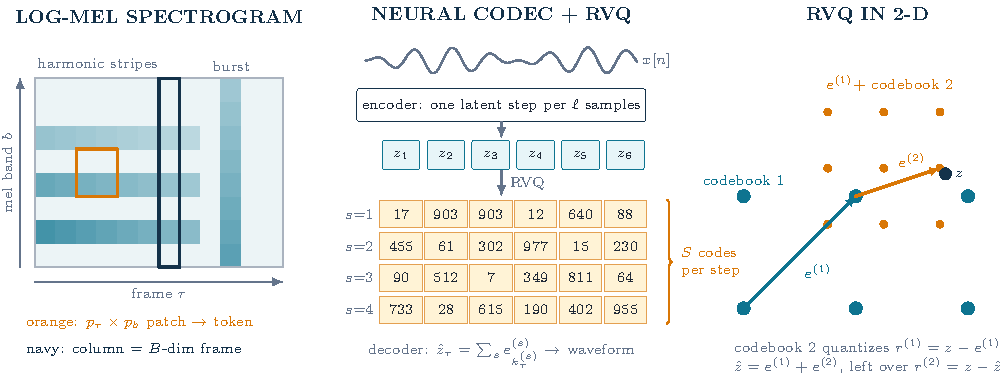
\includegraphics[width=\textwidth]{audio_representations.pdf}
\caption{音频的两种表示。左：对数梅尔频谱，横轴为帧，纵轴为梅尔频带；可以切二维 patch（橙框），也可以逐帧读出 \(B\) 维列向量（深蓝框）。中：编解码器每 \(\ell\) 个采样点输出一个潜在向量 \(z_\tau\)，残差向量量化把它变成 \(S\) 个编号，整段音频成为 \(S\times T\) 的整数网格。右：第一级选出离 \(z\) 最近的 \(e^{(1)}\)，第二级选出离残差 \(r^{(1)}=z-e^{(1)}\) 最近的 \(e^{(2)}\)，两者之和 \(\hat z\) 已接近 \(z\)。}
\label{fig:audio-representations}
\end{figure}

\textbf{对数梅尔频谱。}每隔 \(\ell\) 个采样点取一段长为 \(L\) 的加窗信号做傅里叶变换，把功率谱用 \(B\) 个梅尔滤波器 \(\Phi_{b,\kappa}\) 合并成频带，再取对数：
\begin{equation}
 Y_{\tau,b}=\log\Bigl(\sum_{\kappa}\Phi_{b,\kappa}\,|X_{\tau,\kappa}|^2+\varepsilon\Bigr),
 \qquad
 X_{\tau,\kappa}=\sum_{n=0}^{L-1}x[\tau\ell+n]\,w[n]\,e^{-2\pi\mathrm i\kappa n/L}.
\end{equation}
梅尔频带在低频窄、在高频宽，接近人耳的分辨率。\(Y\) 可以看成一幅图：横轴是帧 \(\tau\)，纵轴是频带 \(b\)，像素值是对数能量。它可以像 ViT 一样切成二维 patch，也可以把每一帧的 \(B\) 维列向量当作一个输入；Whisper 用后一种，每秒 100 帧，经卷积降采样后 30 秒音频成为 1500 个 token~\cite{radford2023whisper}。梅尔频谱丢掉了相位，用于生成时还需要声码器还原波形。

\textbf{神经音频编解码器与残差向量量化。}编解码器的卷积编码器每 \(\ell\) 个采样点输出一个潜在向量 \(z_\tau\)，解码器再把它们还原成波形，两者以重建损失和对抗损失联合训练~\cite{zeghidour2021soundstream,defossez2022encodec}。量化若只用一个含 \(M=1024\) 个码字的码本，每帧只有 10 比特，不足以高保真地重建声音。残差向量量化（Residual Vector Quantization，RVQ）用 \(S\) 个码本逐级量化，每一级量化前面各级留下的残差：
\begin{equation}
 r^{(0)}_\tau=z_\tau,\qquad
 k^{(s)}_\tau=\argmin_{j}\bigl\|r^{(s-1)}_\tau-e^{(s)}_j\bigr\|_2^2,\qquad
 r^{(s)}_\tau=r^{(s-1)}_\tau-e^{(s)}_{k^{(s)}_\tau},
 \qquad
 \hat z_\tau=\sum_{s=1}^{S}e^{(s)}_{k^{(s)}_\tau}.
 \label{eq:rvq}
\end{equation}
图 \ref{fig:audio-representations} 右侧是二维示意：\(z=(1.8,1.2)\)，第一级选中 \((1,1)\)，残差 \((0.8,0.2)\)；第二级选中 \((0.75,0.25)\)，残差缩小为 \((0.05,-0.05)\)。每一级本身就是第 \ref{sec:vector-quantized-latents} 节的向量量化（Vector Quantization，VQ）。每帧由 \(S\) 个编号表示，共 \(S\log_2M\) 比特；EnCodec 每秒 75 帧，取 \(S=8\) 时码率为 6 kbps。整段音频因此是 \(S\times T\) 的编号网格，按帧展开成序列时长度为 \(ST\)。

\textbf{理解用的表示与生成用的表示。}按训练目标，视觉 token 化可以分成两类，见表 \ref{tab:visual-tokenizers}。ViT 或图文对比预训练（Contrastive Language--Image Pre-training，CLIP）的图像编码器用分类或图文对比损失训练，只需保留区分语义所需的信息，没有解码器，输出不能还原成像素；它们是语言模型读取图像的入口。自编码器类 tokenizer，即第 \ref{sec:vector-quantized-latents} 节的 VQ-VAE 和潜空间扩散使用的自编码器，用重建损失训练，必须保留纹理和细节，并配有解码器；它们是生成模型工作的空间。前者擅长回答“图中是什么”，后者能把图画出来。同一套表示很难同时做好这两件事，这是第 \ref{sec:unified-multimodal} 节统一模型的核心难点。重建型 tokenizer 按输出形式又分两种。潜空间扩散的自编码器沿用第 \ref{chap:model-families} 章 VAE 的编码器—解码器结构，文献中通常直接称为 VAE；它输出连续向量网格，扩散直接在这些向量上进行。VQ-VAE 一类在同样的编码器之后再多一步量化，下文简称 VQ tokenizer：编码器把图像压成一个较小的向量网格，每个向量替换成码本中最近的码字，图像就变成一个整数编号网格，例如 \(512\times512\) 的图像变成 \(32\times32\) 个编号，可以像文本 token 一样排成序列做下一 token 预测；配套的解码器把编号网格还原成图像。

\begin{table}[ht]
\centering\small
\begin{tabularx}{\textwidth}{>{\bfseries}p{24mm} X X}
\toprule
 & 语义编码器 & 重建型 tokenizer\\
\midrule
训练目标 & 分类交叉熵或图文对比损失 & 像素重建，常加感知损失与对抗损失\\
输出 & 连续的 patch 向量 & 连续潜变量网格或离散码字网格\\
能否还原像素 & 不能，没有解码器 & 能，由解码器还原\\
保留的信息 & 与类别、文本描述相关的语义 & 纹理、边缘、颜色等局部细节\\
主要用途 & 视觉语言模型的视觉输入、检索、零样本分类 & 潜空间扩散、自回归图像生成\\
典型例子 & ViT、CLIP 图像编码器（第 \ref{sec:clip} 节） &潜空间扩散的自编码器、VQ-VAE\\
\bottomrule
\end{tabularx}
\caption{两类视觉表示。语义编码器服务于理解，重建型 tokenizer 服务于生成。}
\label{tab:visual-tokenizers}
\end{table}

\section{图文对比学习：对齐优化了什么}
\label{sec:clip}

图像向量和文本向量各自可用，但默认不在同一个语义空间。CLIP 通过让配对图文接近、非配对图文分开，建立可比较的表示；它使用一个 image encoder \(f_I\) 和一个 text encoder \(f_T\)，分别把图像 \(I_i\) 和配对文本 \(S_i\) 映射到同一个 \(d_c\) 维空间~\cite{radford2021clip}：
\begin{equation}
 u_i=\frac{f_I(I_i)}{\|f_I(I_i)\|_2},\qquad
 v_i=\frac{f_T(S_i)}{\|f_T(S_i)\|_2},\qquad
 \ell_{ij}=\frac{u_i^\mathsf T v_j}{\tau}.
\end{equation}
一个 batch 中其他图文对的文本就是负样本，\(B\) 个图像和 \(B\) 个文本构成一个 \(B\times B\) 的打分矩阵，对角线是真配对（图 \ref{fig:clip-example} 右）。图像到文本方向的交叉熵把 \(\ell_{ii}\) 推高、把 \(\ell_{ij}\)（\(j\neq i\)）压低；文本到图像方向再做一次对称的交叉熵：
\begin{equation}
 \mathcal L_{\mathrm{CLIP}}
 =\frac12\left[
 -\frac1B\sum_i\log\frac{\exp\ell_{ii}}{\sum_j\exp\ell_{ij}}
 -\frac1B\sum_i\log\frac{\exp\ell_{ii}}{\sum_j\exp\ell_{ji}}
 \right].
 \label{eq:clip-loss}
\end{equation}
归一化把训练重点放在向量间的角度，温度 \(\tau\) 控制相似度分布的尖锐程度。

\begin{figure}[t]
\centering
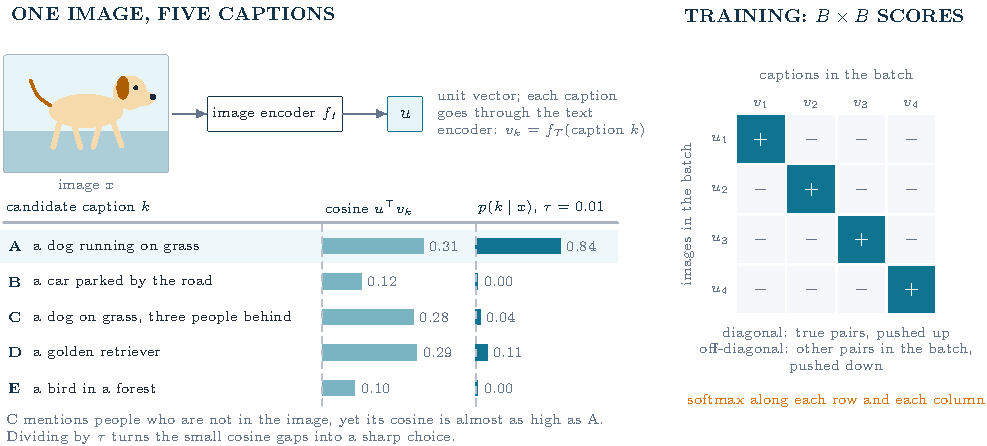
\includegraphics[width=\textwidth]{clip_example.pdf}
\caption{CLIP 在做什么。左：一张狗在草地上奔跑的图像经图像编码器得到 \(u\)，五条候选文本经文本编码器得到 \(v_k\)，逐一计算余弦相似度，再除以温度做 softmax。候选 C 提到了图中没有的三个人，余弦仍与 A 相差无几。右：训练时 batch 内的 \(B\) 张图像与 \(B\) 条文本两两打分，对角线上的真配对被推高，其余被压低。数值为示意。}
\label{fig:clip-example}
\end{figure}

训练完成后，图像与文本可以直接比较。图 \ref{fig:clip-example} 左侧是一个例子：同一张图像与五条候选文本分别计算余弦相似度，正确描述 A 得分最高。各候选的余弦只相差零点几，A 与 D 只差 0.02，但除以 \(\tau=0.01\) 后 logit 相差 2，概率相差约 \(e^2\approx7\) 倍。零样本分类就是这种比较：把每个类别名填进“一张\{类别\}的照片”这样的模板，经文本编码器得到 \(v_k\)，图像属于第 \(k\) 类的概率取为
\begin{equation}
 p(k\mid I)=\frac{\exp(u^\mathsf T v_k/\tau)}{\sum_{k'}\exp(u^\mathsf T v_{k'}/\tau)},
\end{equation}
不需要用这些类别的标注数据训练分类头。CLIP 学到的是整幅图像与整段文本之间的全局对应。它的局限也很明确：不擅长细粒度的空间关系、计数、图中文字和复杂的组合关系。图中候选 C 多出了图里没有的“三个人”，得分却几乎不降，就是这种局限的表现。

\textbf{能量与配分函数。}令 \(E_{ij}=-u_i^\mathsf T v_j\) 为图文对 \((i,j)\) 的能量。图像到文本方向第 \(i\) 行的损失可以写成
\begin{equation}
 \mathcal L_i=-\log\frac{e^{-E_{ii}/\tau}}{Z_i}=\frac{E_{ii}-F_i}{\tau},\qquad
 Z_i=\sum_{j=1}^{B}e^{-E_{ij}/\tau},\qquad
 F_i=-\tau\log Z_i .
\end{equation}
这是一个只有 \(B\) 个候选状态的正则系综：\(\tau\) 是温度，\(Z_i\) 是配分函数，\(F_i\) 是自由能。对参数求导得
\begin{equation}
 \nabla\mathcal L_i=\frac1\tau\Bigl[\nabla E_{ii}-\sum_j p_{ij}\nabla E_{ij}\Bigr],\qquad
 p_{ij}=\frac{e^{-E_{ij}/\tau}}{Z_i}.
\end{equation}
它与第 \ref{sec:ebm-mcmc} 节能量模型的梯度结构相同：第一项是正相位，降低真实配对的能量；第二项是负相位，按玻尔兹曼权重推高各候选配对的能量，与图像越相似的错误文本被推得越多。区别在负样本的来源：能量模型要用 MCMC 从模型分布中采样，CLIP 直接拿 batch 内的其他文本充当负样本，配分函数只在这 \(B\) 个候选上求和。温度越低，\(p_{ij}\) 越集中在最难区分的负样本上；CLIP 把 \(\tau\) 作为可学习参数。

\textbf{互信息下界。}式 \eqref{eq:clip-loss} 是两个方向的平均，这里只看图像到文本方向的那一半，另一方向同理。第 \(i\) 行对 \(B\) 条文本做 softmax，得到的 \(p_{ij}\) 与上一段相同：
\begin{equation}
 p_{ij}=\frac{\exp\ell_{ij}}{\sum_{k=1}^{B}\exp\ell_{ik}},\qquad
 \mathcal L_{\mathrm{InfoNCE}}=-\frac1B\sum_{i=1}^{B}\log p_{ii}.
 \label{eq:infonce}
\end{equation}
\(p_{ij}\) 可以读作模型认为“文本 \(j\) 是图像 \(i\) 的配对”的概率，损失就是真配对拿到的概率取负对数，再对 batch 平均。这种 batch 内 softmax 形式的对比损失称为 InfoNCE~\cite{vandenOord2018cpc}。

于是每一行都是一个猜谜游戏：给定一张图像，把概率分给 \(B\) 条候选文本，真配对分到的越多，损失越小。有两个参照点。全部押中真配对时 \(p_{ii}=1\)，损失为 0；编码器什么都没学到时，只能平均分配，\(p_{ii}=1/B\)，损失为 \(-\log(1/B)=\log B\)。实际损失介于两者之间，\(\log B-\mathcal L_{\mathrm{InfoNCE}}\) 衡量模型比随机猜好多少。例如 \(B=4\) 时（对数取自然对数，下同），随机猜的损失是 \(\log4\approx1.39\)；若模型对每张图像都给真配对 0.9 的概率，损失为 \(-\log0.9\approx0.11\)，比随机猜好 1.28。这个差值不会超过图像与文本之间的互信息：
\begin{equation}
 I(X;Y)\ge\log B-\mathcal L_{\mathrm{InfoNCE}}.
 \label{eq:infonce-bound}
\end{equation}
反过来读：训练把损失降到多少，就证明了图像与文本之间至少有多少互信息，上例中至少为 1.28。

对随机变量 \(Z_1\)，熵 \(H(Z_1)=\E[-\log P(Z_1)]\) 衡量对它的不确定度，在 \(B\) 个取值上均匀分布时为 \(\log B\)；条件熵 \(H(Z_1\mid Z_2)=\E[-\log P(Z_1\mid Z_2)]\) 是已知 \(Z_2\) 后剩下的不确定度。互信息是知道另一组变量后不确定度减少的量：
\begin{equation}
 I(Z_1;Z_2)=H(Z_1)-H(Z_1\mid Z_2),\qquad
 I(Z_1;Z_3\mid Z_2)=H(Z_1\mid Z_2)-H(Z_1\mid Z_2,Z_3).
\end{equation}
记号中分号隔开相比较的两边，逗号把几个变量合成一组，竖线后面是已知条件：\(I(Z_1;Z_2,Z_3)\) 是 \(Z_1\) 与 \((Z_2,Z_3)\) 这一组之间的互信息，条件互信息 \(I(Z_1;Z_3\mid Z_2)\) 是已知 \(Z_2\) 时 \(Z_3\) 还能提供的关于 \(Z_1\) 的信息。两种互信息都非负，且对分号两边对称。由定义直接得到链式法则 \(I(Z_1;Z_2,Z_3)=I(Z_1;Z_2)+I(Z_1;Z_3\mid Z_2)\)：一次看到 \((Z_2,Z_3)\) 得到的信息，等于先看 \(Z_2\) 得到的，加上已知 \(Z_2\) 后再看 \(Z_3\) 新增的。图像 \(X\) 与配对文本 \(Y\) 之间的互信息
\begin{equation}
 I(X;Y)=H(Y)-H(Y\mid X)=\E_{p(x,y)}\log\frac{p(y\mid x)}{p(y)}
\end{equation}
是看到图像后，对配对文本的不确定度平均减少了多少。

直观上，模型比随机猜好的部分只能来自线索，而线索只有一个来源：单看文本，\(B\) 条都像是从语料里随手抽出来的，分不出哪条特别；能把真配对挑出来的，只有它与图像之间的关联，其总量就是 \(I(X;Y)\)。严格地，只看第 \(i\) 行并打乱文本的顺序，softmax 不关心候选的排列，损失不变。于是真配对在一个均匀随机的位置 \(J\)：\((X,Y_J)\) 从 \(p(x,y)\) 中抽出，其余 \(B-1\) 条文本看作从 \(p(y)\) 中独立抽出，这里用大写字母表示随机变量。模型看到 \(D=(X,Y_{1:B})\)，给出猜测 \(q(J=j\mid D)=p_{ij}\)。

第一步，任何猜法都不比真实后验 \(P(J\mid D)\) 更好。交叉熵可以分解为熵加 KL 散度：
\begin{equation}
 \mathcal L_{\mathrm{InfoNCE}}=\E\bigl[-\log q(J\mid D)\bigr]
 =H(J\mid D)+\E_D\,\KL\bigl(P(\cdot\mid D)\Vert q(\cdot\mid D)\bigr)
 \ge H(J\mid D).
\end{equation}

第二步，比随机猜省下的不确定度就是互信息：\(\log B-H(J\mid D)=H(J)-H(J\mid D)=I(J;D)\)。与第一步合起来，\(\log B-\mathcal L_{\mathrm{InfoNCE}}\le I(J;D)\)。

第三步，线索不超过图像与文本共享的信息：
\begin{equation}
 I(J;D)=I(J;X\mid Y_{1:B})\le I(X;J,Y_{1:B})=I(X;Y).
\end{equation}
第一个等号用链式法则 \(I(J;D)=I(J;Y_{1:B})+I(J;X\mid Y_{1:B})\)，单看文本猜不出 \(J\)，\(I(J;Y_{1:B})=0\)。不等号再用一次链式法则，\(I(X;J,Y_{1:B})=I(X;Y_{1:B})+I(X;J\mid Y_{1:B})\)，多出的一项非负。最后一个等号换一种顺序展开，\(I(X;J,Y_{1:B})=I(X;J)+I(X;Y_{1:B}\mid J)\)：位置 \(J\) 与图像无关，第一项为 0；已知 \(J\) 时，与 \(X\) 相关的只有 \(Y_J\)，而 \((X,Y_J)\) 服从 \(p(x,y)\)，第二项等于 \(I(X;Y)\)。三步合起来就是式 \eqref{eq:infonce-bound}~\cite{poole2019variational}。证明没有用到编码器的任何性质；把图像和文本换成两个编码器的输出 \(u,v\)，同样的三步说明 \(\log B-\mathcal L_{\mathrm{InfoNCE}}\) 也是两个表示之间互信息的下界。

第一步的不等式在模型的猜测等于真实后验时取等号，由此可以求出打分 \(\ell_{ij}\) 在最优时学到的量。由贝叶斯公式，
\begin{equation}
 P(J=j\mid D)\propto p(y_j\mid x)\prod_{k\neq j}p(y_k)
 =\frac{p(y_j\mid x)}{p(y_j)}\prod_{k=1}^{B}p(y_k),
\end{equation}
连乘与 \(j\) 无关，所以真实后验正比于 \(p(y_j\mid x)/p(y_j)\)。softmax 的概率正比于 \(e^{\ell_{ij}}\)，两者一致要求打分为
\begin{equation}
 s^*(x,y)=\log\frac{p(y\mid x)}{p(y)}+c(x)=\log\frac{p(x,y)}{p(x)p(y)}+c(x),
\end{equation}
即逐点互信息，再加一个只依赖图像、在 softmax 中会约掉的常数。逐点互信息衡量看到图像后这条文本比平时可信了多少倍，而不是文本本身有多常见，所以“一张照片”这种对任何图像都适用的文本得分不会高。

这个下界给出两条结论。第一，损失非负，下界因而不超过 \(\log B\)：即使损失降到零，也只能证明 \(\log B\) 的互信息。CLIP 使用 32768 的 batch，\(\log B\approx10.4\)，大 batch 不只是加速手段，也决定了目标能分辨多少信息。第二，目标只奖励图像中与配对文本共享的信息。网络文本很少描述物体的精确个数、左右位置或图中小字，这些细节与文本的互信息很小，编码它们几乎不降低损失，全局对比学习也就没有动力保留它们。这正是上面所说的细粒度局限。

\textbf{sigmoid 版本。}语言图像预训练的 sigmoid 损失（Sigmoid Loss for Language Image Pre-training，SigLIP）把每个图文对看成独立的二分类~\cite{zhai2023siglip}：
\begin{equation}
 \mathcal L_{\mathrm{sig}}=-\frac1B\sum_{i,j}\log\sigma\bigl(z_{ij}(t\,u_i^\mathsf T v_j+b)\bigr),\qquad
 z_{ij}=\begin{cases}+1,&i=j,\\-1,&i\neq j,\end{cases}
\end{equation}
其中 \(t\) 是可学习的尺度，\(b\) 是可学习的偏置。它不对整行做 softmax，因而没有配分函数，相似度矩阵可以分块计算，对 batch 大小的依赖也比 softmax 版本小。逻辑回归的最优 logit 同样是逐点互信息，再加上正负样本先验比的对数；一个 batch 中正负样本之比约为 \(1:(B-1)\)，这部分由偏置 \(b\) 吸收，所以 \(b\) 通常初始化为较大的负值。两种损失学到的都是全局相似度接口，都不会自动得到 patch 与词语之间的精确对应。用这种损失训练出的图像编码器通常也直接叫 SigLIP 编码器；它和 CLIP 图像编码器一样是语义编码器，输出 patch 向量，是当前许多视觉语言模型的视觉部分。

\section{视觉语言模型：把视觉 token 接进语言模型}
\label{sec:vlm}

视觉语言模型（Vision--Language Model，VLM）读入一张图像和一段文字，输出文字，例如看图回答“左边是什么”。它的做法是把图像翻译成一串语言模型能读的向量，排在问题前面，让语言模型像读一段特殊的前缀那样读它。图 \ref{fig:vlm-architecture}(a) 画出了这个结构，它由三部分组成。视觉编码器通常就是上一节的 CLIP 或 SigLIP 图像编码器，它把图像切成 patch，为每个 patch 输出一个向量。这里保留全部 patch 向量，而不是只取一个全局向量，因为全局向量丢掉了物体在哪里，回答“左边是什么”恰恰需要空间信息。连接器（connector）通常只是一个小 MLP，把每个 patch 向量映射成语言模型输入空间中的 \(d\) 维向量，得到视觉 token \(v_{1:K}\)，token 数就是第 \ref{sec:visual-tokens} 节的 patch 数。连接器也可以把 token 数压到固定的 \(K\) 个：用 \(K\) 个可学习的 query 向量通过交叉注意力读取全部 patch 向量，每个 query 输出一个视觉 token，图像再大 \(K\) 也不变，BLIP-2 的 Q-Former 就是这样做的~\cite{li2023blip2}，代价是小字之类的细节可能在压缩中丢失。语言模型是一个普通的 decoder-only Transformer，它的输入是视觉 token 后面接文本 token，因果自注意力对两者一视同仁，回答逐 token 生成。

\begin{figure}[t]
\centering
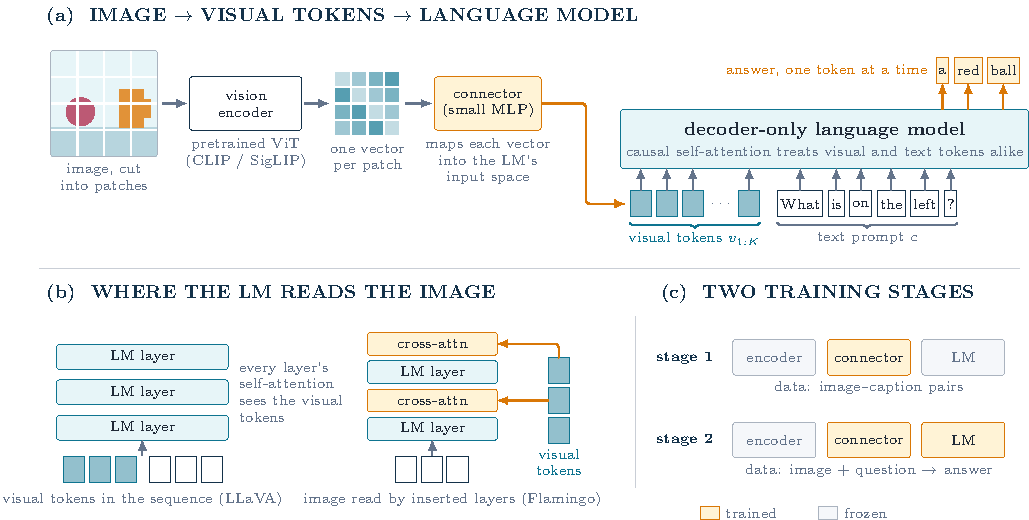
\includegraphics[width=\textwidth]{vlm_architecture.pdf}
\caption{视觉语言模型的结构。(a) 视觉编码器为每个 patch 输出一个向量，连接器把它们映射成视觉 token，排在文本提示前面送进语言模型，语言模型逐 token 生成回答。(b) 语言模型读取图像的两种方式：视觉 token 直接进入输入序列，或者留在序列之外，由插入的交叉注意力层读取。(c) 常见的两阶段训练：先只训练连接器，再连同语言模型一起微调。}
\label{fig:vlm-architecture}
\end{figure}

\textbf{语言模型在哪里读取图像。}图 \ref{fig:vlm-architecture}(b) 是两种方式。第一种是序列拼接：视觉 token 直接作为前缀放进输入序列，语言模型每一层的自注意力都能读到它们。LLaVA（Large Language and Vision Assistant）就是 CLIP 图像编码器加一个投影层，再接语言模型~\cite{liu2023llava}。语言模型的结构完全不变，这是它最大的优点，代价是视觉 token 占用序列长度，也一样写进 KV cache（第 \ref{sec:kv-budget} 节）。第二种是交叉注意力：图像不进入输入序列，而是在语言模型的层之间插入新的交叉注意力层，文字位置的隐状态作 query，视觉 token 作 key 和 value~\cite{alayrac2022flamingo}。它不占序列长度，但要新增层和参数。Flamingo 让每个新层的输出先乘一个初始为零的门控系数，训练开始时模型与原来的语言模型完全相同，之后再逐渐学会看图。

\textbf{训练。}VLM 的损失就是以图像为条件的下一 token 交叉熵：
\begin{equation}
\log p_\theta(y_{1:T}\mid v_{1:K},c)
=\sum_t\log p_\theta(y_t\mid y_{<t},v_{1:K},c),
\end{equation}
其中 \(c\) 是文本提示，\(y\) 是要生成的回答。损失的形式与语言模型相同，学到什么取决于数据，以及哪些部分参与更新。图 \ref{fig:vlm-architecture}(c) 是以 LLaVA 为代表的两阶段流程。第一阶段只训练连接器，视觉编码器和语言模型都冻结，数据是图像和它的描述。这一步相当于为连接器编一本词典，让映射后的视觉向量落在语言模型读得懂的位置。语言模型此时要冻结，因为刚初始化的连接器输出的是噪声，若语言模型跟着更新，已有的语言能力会受损。第二阶段做视觉指令微调，数据是“图像 + 问题 + 回答”，连接器和语言模型一起训练，损失只算在回答 token 上，与第 \ref{chap:training-methods} 章的监督微调（Supervised Fine-Tuning，SFT）相同。

\section{条件图像与视频生成}
\label{sec:conditional-generation}

生成方向把上一节的信息流倒过来：输入文字，输出像素。第 \ref{chap:model-families} 章已经给出了所需的生成算法：潜空间扩散和两种去噪网络（第 \ref{sec:diffusion-score} 节和图 \ref{fig:diffusion-denoiser}）、无分类器引导（式 \eqref{eq:cfg}），以及用 VQ-VAE 码字做自回归生成（第 \ref{sec:vector-quantized-latents} 节）。这一节不重复这些算法，只讨论多模态场景下新增的问题：在哪个表示空间生成，文本条件怎样编码，条件从哪里进入网络，以及视频带来的额外成本。

\textbf{在哪个空间生成。}在像素空间生成，每一步都要处理整幅图像。潜空间扩散先用表 \ref{tab:visual-tokenizers} 中的重建型自编码器把图像压成小得多的潜变量，例如 \(512\times512\times3\) 压成 \(64\times64\times4\)，去噪网络只在潜空间工作，细节由解码器补回~\cite{rombach2022ldm}。压缩率越高，生成越便宜，但解码器的重建质量成了整个系统的上限：自编码器还原不出的小字或细纹理，生成模型也画不出来。这也是这类自编码器要加感知损失和对抗损失的原因：只用像素均方误差训练时，解码器会对一组同样合理的细节取平均，重建就发糊~\cite{esser2021vqgan}。

\textbf{离散 token 的生成顺序。}若 tokenizer 输出离散码字，图像生成就成了序列生成。按光栅顺序逐个预测码字，可以直接复用语言模型，但一张 \(32\times32\) 的码字网格需要 1024 次串行调用，而且左上角生成时看不到右下角。MaskGIT 改为并行生成：从全部遮住开始，每一轮预测所有被遮住的位置，保留最有把握的一部分，其余重新遮住，约 8 轮即可完成~\cite{chang2022maskgit}。这就是第 \ref{sec:discrete-diffusion} 节的离散掩码扩散。

\textbf{文本条件怎样编码。}文本先经过一个通常冻结的文本编码器，得到一串 token 向量。早期的潜空间扩散使用 CLIP 文本编码器。Imagen 改用只在文本上预训练的 T5（Text-to-Text Transfer Transformer）编码器，发现增大文本编码器比增大扩散网络更能提高图文一致性~\cite{saharia2022imagen}。第 \ref{sec:clip} 节的互信息分析给出了解释：CLIP 文本编码器只被训练去保留有助于全局匹配的信息，对词序、数量和属性归属不敏感，比如分不清“红色的方块和蓝色的球”中哪个颜色属于哪个物体；在大量文本上训练的语言模型保留了更多句法结构。所以许多模型同时使用两类编码器~\cite{esser2024sd3}。

\textbf{条件从哪里进入网络。}文本 token 向量进入去噪网络有三种方式，前两种与上一节 VLM 的两种读取方式相同。交叉注意力让图像位置作 query、文本 token 作 key 和 value，U-Net 类去噪网络这样做（图 \ref{fig:diffusion-denoiser}）。序列拼接把文本 token 和图像 patch token 拼成一条序列做联合注意力，Stable Diffusion 3（SD3）这样做~\cite{esser2024sd3}。归一化调制把时间步、类别等条件压成一个向量，由它生成每层归一化的缩放和平移参数，DiT 用它注入时间步和类别标签~\cite{peebles2023dit}。前两种方式让每个图像位置都能读取每个文本 token，适合表达“左边红色、右边蓝色”这类逐位置的描述；调制对整幅图像施加同一组参数，只能表达全局属性，但最便宜。表 \ref{tab:condition-interfaces} 把理解与生成两个方向的注入方式放在一起比较。

\textbf{空间条件与编辑。}深度图、边缘图、人体姿态这类条件与图像处在同一空间网格上，可以逐位置对应，最简单的做法是把它们缩放到潜变量的分辨率，与带噪潜变量按通道拼接作为输入。修复就是这样做的：把掩码和保留区域拼进输入，模型只生成掩码内的内容。ControlNet 则不改动原网络：冻结预训练的去噪网络，复制一份可训练的分支读取条件图，分支的输出经初始化为零的卷积加回原网络~\cite{zhang2023controlnet}。训练开始时输出与原模型完全相同，这与 Flamingo 的零初始化门控是同一个思路：新加的条件通路从不起作用开始学，不破坏预训练得到的能力。

\textbf{视频。}视频生成在图像的基础上增加时间轴，成本主要来自 token 数。视频自编码器同时压缩空间和时间，但一段 4 秒的视频仍有同分辨率单张图像约 24 倍的 token。扩散的每一步都要对全部 token 做双向注意力，代价按 token 数的平方增长，24 倍的 token 意味着约 576 倍的注意力计算。常见的折中是分解注意力：一些层只在帧内做空间注意力，另一些层只在同一位置的不同帧之间做时间注意力，代价降为两部分之和，但跨帧、跨位置的交互要经过多层间接传递。让物体在运动中保持外观和形状一致，是视频生成相对图像生成新增的主要难点。

\begin{table}[ht]
\centering\small
\begin{tabularx}{\textwidth}{>{\bfseries\raggedright\arraybackslash}p{19mm} >{\raggedright\arraybackslash}X >{\raggedright\arraybackslash}p{22mm} >{\raggedright\arraybackslash}p{22mm} >{\raggedright\arraybackslash}X}
\toprule
接口 & 条件怎样进入 & 理解方向 & 生成方向 & 代价与表达能力\\
\midrule
序列拼接 & 条件 token 与主序列拼接，共用 self-attention & LLaVA、BLIP-2 的视觉前缀 & SD3 的文图联合注意力 & 序列变长，注意力按总长度平方增长；逐 token 双向交互\\
交叉注意力 & 主序列作 query，读取条件的 key 和 value & Flamingo & U-Net 读取文本 & 不占主序列长度，但增加层；条件表示不随主序列更新\\
归一化调制 & 条件压成一个向量，生成缩放、平移和门控参数 & 少用 & DiT 的时间步与类别 & 最便宜；只能表达全局属性\\
通道拼接 & 条件与输入逐位置对齐，按通道拼接 & 少用 & 修复掩码、深度图 & 要求同一空间网格；逐位置控制\\
全局相似度 & 两个编码器只在输出向量处比较 & CLIP 检索、零样本分类 & 不适用 & 最便宜；无细粒度交互，不能生成\\
\bottomrule
\end{tabularx}
\caption{条件注入接口。理解与生成两个方向共用前两种接口；它们的差别在于条件以多少个 token 出现，以及主网络在哪里读取它。}
\label{tab:condition-interfaces}
\end{table}

\section{统一多模态模型：理解与生成放进一个网络}
\label{sec:unified-multimodal}

前两节的理解模型和生成模型是分开的：VLM 读取语义编码器的输出，写出文字；图像生成模型在重建型潜空间中写出图像。统一模型想用一个 Transformer 在同一段上下文中既读又写，例如看图回答问题之后接着画一张修改后的图。设计时要回答两个问题。第一，读图和画图是否用同一种图像表示：语义编码器便于理解但不能还原像素，重建型 tokenizer 能画图但语义较弱（表 \ref{tab:visual-tokenizers}）。第二，图像以什么方式生成：VQ 码字可以像文字一样做下一 token 预测，连续的 VAE 潜变量则用扩散去噪。图 \ref{fig:unified-routes} 是三种有代表性的回答。

\begin{figure}[!tb]
\centering
\begin{tikzpicture}[x=1cm,y=1cm,font=\small,
  ttok/.style={draw=Teal,fill=Sky,minimum size=3.2mm,inner sep=0pt},
  dtok/.style={draw=Orange,fill=Amber,minimum size=3.2mm,inner sep=0pt},
  ctok/.style={circle,draw=Orange,fill=Amber,minimum size=3.2mm,inner sep=0pt},
  ubox/.style={draw=Navy,fill=white,rounded corners=2pt,minimum width=46mm,minimum height=9mm,align=center,font=\footnotesize},
  hbox/.style={ubox,minimum width=21mm},
  trunk/.style={ubox,fill=Mist},
  head/.style={font=\small\bfseries,color=Navy},
  cost/.style={font=\scriptsize,color=Slate,align=center}]
\begin{scope}
  \node[head] at (2.4,5.45) {(a) 全部离散化};
  \node[cost] at (2.4,5.05) {Chameleon};
  \node[ubox] (oa) at (2.4,4.25) {下一 token 预测\\图像码字 \(\to\) VQ 解码器};
  \node[trunk] (ta) at (2.4,2.95) {Transformer\\因果注意力};
  \foreach \i/\s in {0/ttok,1/ttok,2/ttok,3/dtok,4/dtok,5/dtok,6/dtok,7/ttok,8/ttok}
    \node[\s] at ({0.6+0.45*\i},1.75) {};
  \node[ubox] at (2.4,0.6) {VQ 编码器\\读图、画图共用};
  \draw[flow] (2.625,1.05)--(2.625,1.55);
  \draw[flow] (2.4,1.95)--(ta.south);
  \draw[flow] (ta.north)--(oa.south);
  \node[cost] at (2.4,-0.2) {理解只能依赖重建型码字};
\end{scope}
\begin{scope}[xshift=5.4cm]
  \node[head] at (2.4,5.45) {(b) 读写分用两种编码器};
  \node[cost] at (2.4,5.05) {Janus};
  \node[ubox] (ob) at (2.4,4.25) {下一 token 预测\\图像码字 \(\to\) VQ 解码器};
  \node[trunk] (tb) at (2.4,2.95) {Transformer\\因果注意力};
  \foreach \i/\s in {0/ttok,1/ctok,2/ctok,3/ctok,4/ttok,5/ttok,6/dtok,7/dtok,8/dtok,9/ttok}
    \node[\s] at ({0.51+0.42*\i},1.75) {};
  \node[hbox] at (1.2,0.6) {SigLIP 编码器\\用于读图};
  \node[hbox] at (3.6,0.6) {VQ 编码器\\用于画图};
  \draw[flow] (1.35,1.05)--(1.35,1.55);
  \draw[flow] (3.45,1.05)--(3.45,1.55);
  \draw[flow] (2.4,1.95)--(tb.south);
  \draw[flow] (tb.north)--(ob.south);
  \node[cost] at (2.4,-0.2) {同一张图有两种互不相同的表示};
\end{scope}
\begin{scope}[xshift=10.8cm]
  \node[head] at (2.4,5.45) {(c) 文字自回归，图像扩散};
  \node[cost] at (2.4,5.05) {Transfusion};
  \node[ubox] (oc) at (2.4,4.25) {文本：下一 token 预测\\图像：去噪 \(\to\) VAE 解码器};
  \node[trunk] (tc) at (2.4,2.95) {Transformer\\因果注意力，图内双向};
  \foreach \i/\s in {0/ttok,1/ttok,2/ttok,3/ctok,4/ctok,5/ctok,6/ctok,7/ttok,8/ttok}
    \node[\s] at ({0.6+0.45*\i},1.75) {};
  \node[ubox] at (2.4,0.6) {VAE 编码器，不量化\\读图、画图共用};
  \draw[flow] (2.625,1.05)--(2.625,1.55);
  \draw[flow] (2.4,1.95)--(tc.south);
  \draw[flow] (tc.north)--(oc.south);
  \node[cost] at (2.4,-0.2) {逐 token 解码与多步去噪交替进行};
\end{scope}
\node[ttok] at (3.2,-0.8) {};
\node[anchor=west,font=\footnotesize] at (3.4,-0.8) {文本 token};
\node[dtok] at (5.9,-0.8) {};
\node[anchor=west,font=\footnotesize] at (6.1,-0.8) {离散图像码字};
\node[ctok] at (8.9,-0.8) {};
\node[anchor=west,font=\footnotesize] at (9.1,-0.8) {连续图像向量};
\end{tikzpicture}
\caption{三种统一多模态模型。每栏自下而上：编码器把图像变成 token，与文本 token 拼成一条序列送入同一个 Transformer，顶部是训练目标和图像解码方式，最下方一行是主要代价。方块表示离散码字，圆点表示连续向量；VQ 编码器与 VAE 编码器的区别只在输出是否量化成码字（第 \ref{sec:visual-tokens} 节）。}
\label{fig:unified-routes}
\end{figure}

Chameleon 对两个问题都选统一：图像用 VQ 码字表示并入文本词表，读写都是下一 token 预测~\cite{chameleon2024}。图像从第一层起就与文字共享全部参数，没有独立的视觉编码器，这就是“早期融合”。代价是理解只能依赖语义较弱的重建型码字；图像 token 与文本 token 的统计性质差别也大，训练要靠查询与键归一化（Query--Key Normalization，QK-Norm；见第 \ref{sec:qk-norm} 节）等手段维持稳定。Janus 在第一个问题上分开：读图用 SigLIP 编码器（第 \ref{sec:clip} 节），画图仍预测 VQ 码字，代价是同一张图在模型中有两种表示~\cite{wu2024janus}。Transfusion 在第二个问题上改用扩散：图像以不量化的 VAE 潜变量进出网络，文本用下一 token 损失，图像用去噪损失；同一张图内部的 patch 互相可见，因为扩散一次去噪整幅图像~\cite{zhou2024transfusion}。它避开了量化损失，代价是推理时要在逐 token 解码与多步去噪之间切换。

原生多模态模型可以把同样的思路推广到语音：直接读写音频编解码器 token（第 \ref{sec:visual-tokens} 节），在文本、图像和音频上端到端训练。与“语音识别、语言模型、语音合成”三段级联的系统相比，语气、情绪和背景声不会在转写成文字时丢失，延迟也更低。
